\section{Machine Learning Model for Seed Selection}
\label{sec:seed-model}
To train and test the seed-selection model, we use the target expressions
and sufficient seed sets constructed in Section~\ref{sec:integrals-generation}.
We have implemented a small neural network that assigns a binary decision and its estimated confidence
to each supplied candidate seed. We trained the model on the fixed training division and then
evaluated it on the held-out targets. This section defines the inputs,
probabilities and training procedure, and
Section~\ref{sec:seed-test-results} gives the resulting seed predictions.

\subsection{Model inputs and seed probabilities}
\label{sec:seed-model-architecture}
A seed specifies an integral index vector at which the solver generates
IBP identities. The resulting equations can contain other integrals whose
elimination uses identities from additional seed vectors~\cite{KiraOriginal}.
A target can therefore use several seeds in a sufficient reduction set.
Some targets admit a reduction from one seed, while a target already
expressed in the chosen masters needs no IBP seed. We formulate the
prediction as a separate binary decision for every candidate, so the
model can select several seeds for the same target.

For a fixed family and chosen master basis, write a target as
\begin{equation}
 \mathcal T=\sum_{j=1}^{n_T}c_j(\boldsymbol x,d)
                         I_{\boldsymbol a^{(j)}},
 \qquad
 \mathcal C=\{\boldsymbol\sigma_1,\ldots,
                          \boldsymbol\sigma_{n_C}\}.
 \label{eq:seed-model-input}
\end{equation}
Here $n_T$ is the number of terms in the target, $c_j$ is the
rational coefficient of its $j$th term, $\boldsymbol x$ is the
set of kinematic parameters and $d$ is the space-time dimension.
The vector $\boldsymbol a^{(j)}$ gives the integral indices of that
term. The set $\mathcal C$ contains $n_C$ candidate seed vectors
within the stored family bounds. It supplies all candidates that
this implementation scores for the target. Extending the seed bounds
would require supplying an enlarged candidate set.

The model receives every term in the stored order, including its
indices and symbolic coefficient. Each integral contributes its index
values, the locations of positive indices and the quantities $r,s,t$
and $n_{\rm dot}$ defined in Eq.~\eqref{eq:complexities}.
We transform an index value $a$ to
$\operatorname{sgn}(a)\log(1+|a|)$ and transform the nonnegative
counts with $\log(1+v)$, where $v$ denotes the count. The input
also records the number of family indices and which positions are
present. The current representation has capacity for 16 indices;
the existing families use at most five.

To include the coefficient functions, we separate their written
expressions into variable names, integers and mathematical symbols.
We encode counts of individual symbols and consecutive groups of
two and three symbols in a fixed vector with 64 components.
A fixed signed assignment maps each group to a component, and division
by the square root of the total number of groups sets the scale.
Every coefficient symbol enters this representation, although
different groups can share a component. The resulting vector is a
compressed description of the coefficient expression. It does not
perform symbolic simplification or establish equality between
different expressions. In particular, modular residues do not enter
as ordinary real coefficient values.

For each term we append its relative position in the stored list and
the inverse term count. Denote the resulting term vector by
$\boldsymbol f_j$. A shared learned map $\phi_\theta$ forms
\begin{equation}
 \boldsymbol h_j=\phi_\theta(\boldsymbol f_j),
 \qquad \boldsymbol h_j\in\mathbb R^{32}.
 \label{eq:seed-term-embedding}
\end{equation}
Here $\theta$ denotes the adjustable parameters of the model and
$\boldsymbol h_j$ is a vector describing the term. The same map
acts on each term, so its number of parameters does not depend on
$n_T$. Combining shared term maps through averages follows the
set-based construction of Ref.~\cite{DeepSets}, with additional
position information to retain the stored order.

We also include every ordered pair of distinct terms. If $n_T>1$,
their combined description is
\begin{equation}
 \boldsymbol h_{\rm pair}
 =\frac{1}{n_T(n_T-1)}
   \sum_{\substack{j,k=1\\j\ne k}}^{n_T}
   \psi_\theta\!\left(
      [\boldsymbol h_j,\boldsymbol h_k,
       \boldsymbol h_j-\boldsymbol h_k,
       \boldsymbol h_j\odot\boldsymbol h_k]\right).
 \label{eq:seed-pair-embedding}
\end{equation}
Square brackets join vectors, $\odot$ multiplies corresponding
components, and $\psi_\theta$ maps each joined vector to 32 components.
For an individual-integral target, we set
$\boldsymbol h_{\rm pair}=\boldsymbol0$. This representation includes
both orders of each pair and the positions of the associated terms.
The present model uses pairs as its specified form of term combinations;
it does not enumerate longer subsets or all permutations of the full
expression. The fixed stored term order must also be used when preparing
later inputs.

The family information includes the propagator expressions, masses,
external scalar products, invariant names, and the numbers of loops,
propagators, external momenta and invariant parameters. We encode its
symbolic structure
with the same fixed 64-component rule and map it to a 32-component
family vector $\boldsymbol h_F$. A further shared map acts on the
index vectors of the chosen masters, and their mean gives the
32-component basis vector $\boldsymbol h_M$. This input identifies
the basis available for reduction. The target's master coefficients,
construction history and recorded seed choices remain outside the
input.

Each candidate seed contributes its index and complexity information
through a shared map that gives a vector
$\boldsymbol u_b\in\mathbb R^{32}$ for candidate $b$.
To associate a seed with particular target terms, we form
\begin{equation}
 \begin{aligned}
 \omega_{bj}
 &=\frac{\exp(\boldsymbol u_b\cdot\boldsymbol h_j/\sqrt{32})}
         {\sum_{k=1}^{n_T}
           \exp(\boldsymbol u_b\cdot\boldsymbol h_k/\sqrt{32})},\\
 \boldsymbol v_b&=\sum_{j=1}^{n_T}\omega_{bj}\boldsymbol h_j .
 \end{aligned}
 \label{eq:seed-term-attention}
\end{equation}
The weight $\omega_{bj}$ determines how much term $j$ contributes to
candidate $b$'s description, and $\boldsymbol v_b$ is their weighted
mean. This uses the scaled dot-product weighting of
Ref.~\cite{AttentionIsAllYouNeed}. The weights sum to one over target
terms for each seed.

The model then joins the mean and componentwise maximum of the term
vectors with the pair, family, basis, seed and weighted-term vectors:
\begin{equation}
 \begin{aligned}
 \boldsymbol z_b&=[
   \operatorname{mean}_j\boldsymbol h_j,\,
   \operatorname{max}_j\boldsymbol h_j,\,
   \boldsymbol h_{\rm pair},\boldsymbol h_F,\boldsymbol h_M,\,
   \boldsymbol u_b,\boldsymbol v_b],\\
 g_b&=F_\theta(\boldsymbol z_b),\qquad
 p_b=\frac{1}{1+\exp(-g_b)}.
 \end{aligned}
 \label{eq:seed-probability}
\end{equation}
Here $F_\theta$ has a hidden layer with 64 components and one scalar
output $g_b$. The other learned maps each use one layer with 32
components. All hidden layers use the hyperbolic tangent function.
The implementation has 28,097 adjustable parameters
and shares them across candidates, so reordering the candidate list
only reorders the returned scores.

The quantity $p_b$ represents the model's probability that
$\boldsymbol\sigma_b$ belongs to the recorded sufficient seed set.
Several seeds can contribute to the same reduction, so these
probabilities are separate and need not sum to one.
A high score ranks a seed for selection.
The current data establish a valid reference set for each target;
they do not establish the probability that a seed belongs to a
globally minimal reduction. Exact reduction remains the criterion
for deciding whether the selected seeds supply enough equations.

For each candidate we report probabilities for both possible labels:
\begin{equation}
 \begin{aligned}
 P_\theta(y_b=1\mid\mathcal T,F,\mathcal M,\boldsymbol\sigma_b)&=p_b,\\
 P_\theta(y_b=0\mid\mathcal T,F,\mathcal M,\boldsymbol\sigma_b)&=1-p_b.
 \end{aligned}
 \label{eq:seed-class-probabilities}
\end{equation}
Here $y_b$ is the reference label, $F$ is the family definition and
$\mathcal M$ is the chosen master basis. Label 1 means membership in the recorded sufficient seed set.
Label 0 means absence from that set. The two class probabilities for
one seed sum to one, while probabilities for different seeds remain
separate.

The binary prediction uses a fixed threshold of one half:
\begin{equation}
 \widehat y_b=
 \begin{cases}
  1,&p_b\geq\tfrac12,\\
  0,&p_b<\tfrac12.
 \end{cases}
 \qquad
 q_b=\widehat y_b p_b+(1-\widehat y_b)(1-p_b).
 \label{eq:seed-binary-confidence}
\end{equation}
The value $\widehat y_b$ is the returned label, and $q_b$ is the model's
estimated probability that this label agrees with the reference label.
For example, $p_b=0.90$ gives label 1 with confidence $q_b=0.90$,
while $p_b=0.08$ gives label 0 with confidence $q_b=0.92$.
These values illustrate the output rule; they are not trained results.
Candidate selection uses $p_b$, while $q_b$ describes confidence in
the returned binary decision.

The predicted seed set is
\begin{equation}
 \widehat{\mathcal S}(\mathcal T)
   =\{\boldsymbol\sigma_b\in\mathcal C:\widehat y_b=1\}.
 \label{eq:seed-predicted-set}
\end{equation}
Its size can vary between targets. Exact reduction must establish
whether the identities from this set suffice to reduce the target.
The probability $q_b$ concerns one reference-membership decision;
it is not a probability that the complete selected set gives a valid
or minimum-cost reduction. Section~\ref{sec:seed-test-results} compares these confidence values
with their observed agreement with the reference labels.

\subsection{Training labels and the 70:30 data division}
\label{sec:seed-model-split}
For each target, let $\mathcal S_{\mathcal T}\subseteq\mathcal C$
be its recorded sufficient seed set. We define one label per candidate:
\begin{equation}
 y_b(\mathcal T)=
 \begin{cases}
  1,&\boldsymbol\sigma_b\in\mathcal S_{\mathcal T},\\
  0,&\boldsymbol\sigma_b\notin\mathcal S_{\mathcal T}.
 \end{cases}
 \label{eq:seed-membership-label}
\end{equation}
A zero label records absence from this particular set. Another
valid reduction can still use that seed. Targets with empty reference
seed sets retain zero labels for all candidates, and their checks
are kept separate when a comparison requires at least one positive
label.

We assign each complete target, its candidate list and all its labels
to one side of the 70:30 division. We also keep each complete family
together and group four-propagator families with the same kinematic
zero and equality pattern across all mass assignments. This includes
matching patterns among the original massless boxes.
These conditions prevent related targets from the same full family
profile from being used on both sides.

A reproducible assignment gives 168,330 training targets in
693 families and 72,142 test targets in
307 families. The training fraction is 69.99983\%.
The ratio refers to complete target examples; each example carries its
whole seed-label vector, whose length depends on the family.
This model-specific division uses the complete collection and leaves
the original data divisions in Section~\ref{sec:integrals-generation}
available as provenance. Shared lower-sector integrals can still
occur across the two sets. We assigned two complete two-loop families to training and one to
 testing with the fixed split seed. These three families alone cannot establish performance at high
loop orders.

The training objective is the average binary cross-entropy,
\begin{equation}
 \mathcal L(\theta)
 =-\frac{1}{|\mathcal D_{\rm train}|}
  \sum_{\mathcal T\in\mathcal D_{\rm train}}
  \frac{1}{n_C(\mathcal T)}
  \sum_{b=1}^{n_C(\mathcal T)}
  \left[y_b\log p_b+(1-y_b)\log(1-p_b)\right].
 \label{eq:seed-training-loss}
\end{equation}
Here $\mathcal D_{\rm train}$ is the training target set and
$n_C(\mathcal T)$ is the candidate count for that target.
Each target has equal weight in this objective. We retain all candidate
labels and use no additional positive-class weighting. We trained the model with AdamW~\cite{AdamW}, with an initial learning
rate of $10^{-3}$, weight decay of $10^{-4}$ and ten passes through the
training data. We fixed these settings before using the test set.
Training completed all ten passes and made 210,420 parameter updates
from 1,683,300 target presentations. The final saved parameters define
the model used throughout the test.

For example, suppose five candidate seeds accompany a target and its
recorded sufficient set contains the first and third seeds. The label
vector is then
\begin{equation}
 \boldsymbol y(\mathcal T)=(1,0,1,0,0).
 \label{eq:seed-label-example}
\end{equation}
The model receives the target, public family information, chosen basis
and all five candidate seeds. Their labels enter the comparison with
the predictions after the forward calculation; the labels and the
target's master expansion remain outside the model input.

Starting from randomly initialized parameters, the model produces a
probability for every candidate in a training example. A reference
label of 1 contributes $-\log p_b$ to the loss, while a label of 0
contributes $-\log(1-p_b)$. The loss uses these continuous probabilities
during parameter updates. The threshold in
Eq.~\eqref{eq:seed-binary-confidence} applies when reporting decisions.

We differentiate the loss with respect to the model parameters and
average the gradients from eight targets before each update. A gradient
describes how a change in a parameter changes the loss. The training
procedure limits the combined gradient norm to one and uses AdamW to
update the 28,097 parameters. The last group in a pass uses its actual
number of targets when fewer than eight remain. The training examples
change order between passes. Ten passes use each training target ten
times, and the saved parameters after the final pass define the model
for the test comparison. The held-out targets do not enter parameter
updates or threshold selection.

\subsection{Completed training and implementation checks}
Training began from randomly initialized parameters and completed
the fixed ten-pass schedule. The mean loss recorded during the first
pass was 0.0111521, and the mean during the last pass was 0.00148954.
Figure~\ref{fig:training-loss} shows the recorded loss for each pass.
These values average the losses encountered as the parameters changed
within that pass. They describe the training history and do not measure
performance on unseen targets.

\begin{figure}[htbp]
 \centering
 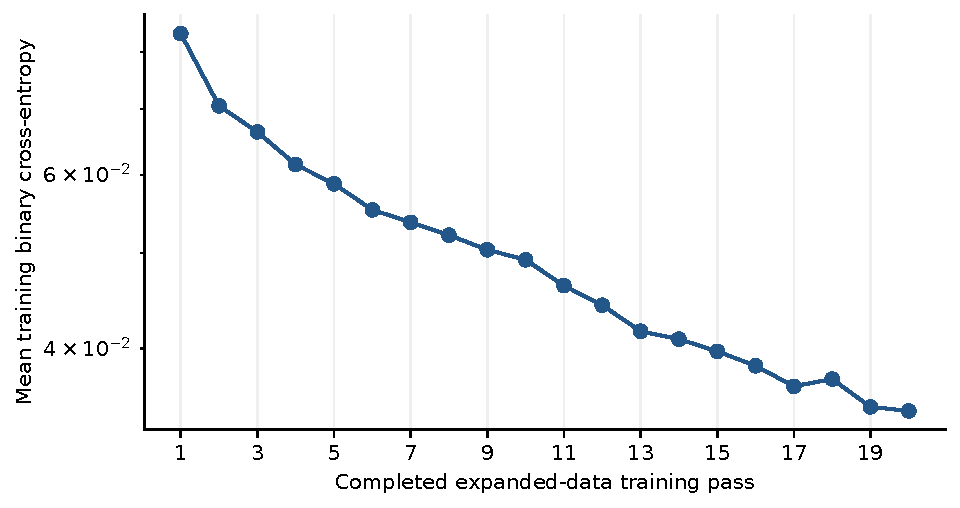
\includegraphics[width=0.80\linewidth]{figures/training_loss.pdf}
 \caption{Mean training binary cross-entropy during each of the ten
 passes. Each training target contributes equal weight to the mean.
 The vertical axis uses a logarithmic scale. The curve records losses
 during parameter updates; it is not a validation curve.}
 \label{fig:training-loss}
\end{figure}

Before training, the preparation checked every target-label
correspondence and verified that every recorded seed appears in its
candidate pool. Implementation checks verified the binary labels, both
class probabilities, the confidence values and the parameter derivatives.
They also confirmed that the input retains coefficient and term-order
information and that a reordering of candidates only reorders their
scores. During training, the held-out targets supplied no parameter
updates, threshold choices or stopping decisions.

The implementation reads examples in bounded groups and scores
candidate seeds and ordered term pairs in blocks. It retains every
ordered pair in Eq.~\eqref{eq:seed-pair-embedding}, so the pair count
grows as $n_T(n_T-1)$. The current bounds are 512 terms, 10,000 candidates
and 16 indices per integral. Inputs beyond these bounds are rejected.
The trained model now permits a direct comparison of its predicted
seed sets with the recorded sets in the separate test collection.
\FloatBarrier
